\newpage
\hypertarget{remCard tex}{}
\subsection{Implementing removeCard}
\texHeader

\begin{itemize}

\item[$\blacktriangleright$] Go to the \texttt{removeCard} signature in \texttt{Partition.eclass}. Complete the method with a single pattern
(\texttt{[deleteSingleCard]}) and a return statement as depicted in Fig~\ref{fig:remCardDec}. We hope you haven't forgotten about eMolfon's type completion; you
can press \texttt{ctrl + space} on an empty line to select and generate a generic pattern template.


\begin{figure}[htp]
\begin{center}
  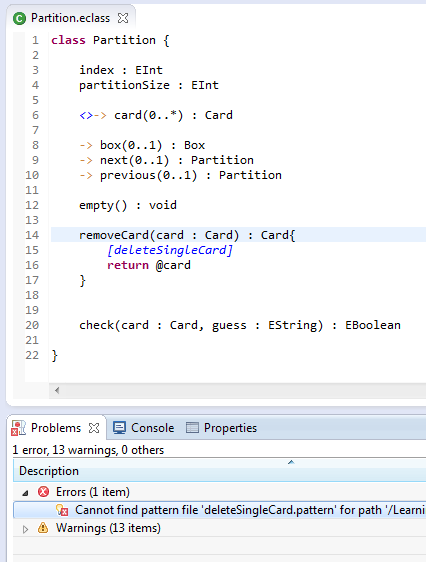
\includegraphics[width=0.5\textwidth]{eclipse_removeCardDeclaration}
  \caption{Control flow for \texttt{removeCard}}
  \label{fig:remCardDec}
\end{center}
\end{figure}

\item[$\blacktriangleright$] This updated construct is refered to as an \emph{activity}. MOSL limits method defintions to just the method's control flow, which
makes this the rule's top layer. All actual transformations are modeled in a separate \emph{patterns} file. In this case, \texttt{removeCard}'s link
deletion will be modeled in \texttt{[deleteSingleCard]}.

\item[$\blacktriangleright$] Save the file, and an error should immediately appear. In the ``Problems'' tab below the editor, the message states that
the builder cannot find the specified pattern file. Well, that makes sense - you haven't made it yet! 

\item[$\blacktriangleright$] Click this message then press \texttt{ctrl + 1} to invoke a ``Quick Fix'' dialouge (Fig~\ref{fig:quixFix}). It offers to create a
pattern file for you. Given that's exactly what you'd like to do, select the option and press \texttt{Finish}.

\begin{figure}[htp]
\begin{center}
  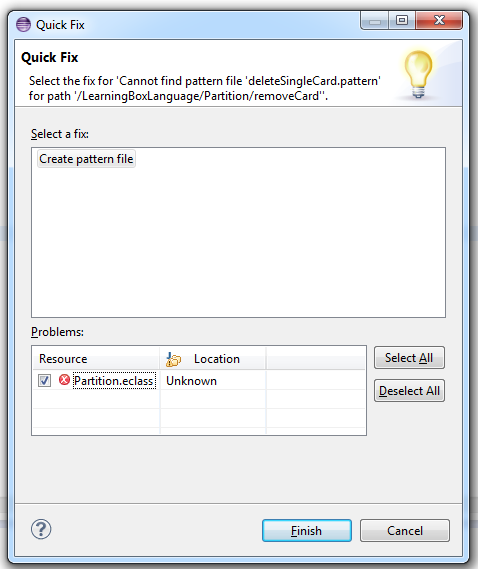
\includegraphics[width=0.6\textwidth]{eclipse_patternQuickFix}
  \caption{A quick solution to a pattern error}
  \label{fig:quixFix}
\end{center}
\end{figure}

\newpage

\item[$\blacktriangleright$] The new file will open in the editor, and you'll be able to see a new directory structure will under
``LearningBoxLanguage/\_patterns'' (Fig.~\ref{fig:pattStruct}). SDMs are placed in SDM containers, named according to the method they implement. In this case,
\texttt{deleteSingleCard.pattern} is invoked by the method \texttt{removeCard}, which itself is found in the \texttt{Partition} EClass. \texttt{Partition} will
eventually contain a folder for each method that needs a pattern.

\vspace{0.5cm}

\begin{figure}[htp]
\begin{center}
  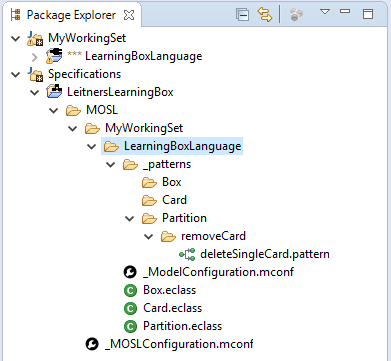
\includegraphics[width=0.9\textwidth]{eclipse_patternStructure}
  \caption{Directory structure for a pattern}
  \label{fig:pattStruct}
\end{center}
\end{figure}

\item[$\blacktriangleright$] The content of any pattern file is simply a list of tasks and rules. You create a series of \emph{object variables}, and then,
within those declarations, state operations such as `delete this reference.' Remember - the main goal of SDMs is to focus here is not on \emph{how}, but
\emph{what}.

\vspace{0.5cm}

\item[$\blacktriangleright$] Create two object variables, \texttt{@this:Partition\{ \}} and~\texttt{@card:Card\{ \}}~(Fig.~\ref{fig:remCardObjVar}). In MOSL
syntax, `\texttt{@}' indicates that a variable is \emph{bounded}.

\begin{figure}[htp]
\begin{center}
  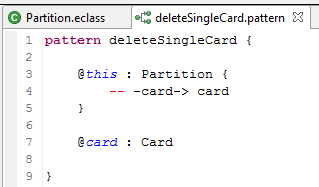
\includegraphics[width=0.6\textwidth]{eclipse_remCardObjVars}
  \caption{Object variables for \texttt{removeCard}}
  \label{fig:remCardObjVar}
\end{center}
\end{figure}

\clearpage

\item[$\blacktriangleright$] Add `\texttt{-- -> card:card}' to \texttt{@this} to destroy the \texttt{card} reference targeting the \texttt{card} object.
Your pattern should now resemble Fig.~\ref{fig:deleteReference}.

\vspace{0.5cm}

\begin{figure}[htp]
\begin{center}
  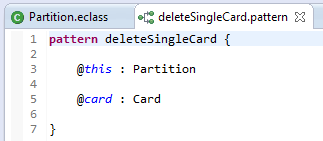
\includegraphics[width=0.6\textwidth]{eclipse_thisObjVar}
  \caption{Destroy the link between a card and its partition}
  \label{fig:deleteReference}
\end{center}
\end{figure}

\item[$\blacktriangleright$] If you ever need to quickly remind yourself of specific navigation names or attributes, press \texttt{alt} and the left arrow to
jump back to your EClass. Conversely, to quickly open or jump to a pattern, Hover over the pattern name while holding \texttt{ctrl} until it's underlined,
then click!

\vspace{0.5cm}

\item[$\blacktriangleright$] Remember that links between classes are defined via \emph{Bidrectional EReferences},\footnote{technically two
\emph{unidirectional EReferences}} linked together as opposites in ``LearningBoxLanguage/\_con\-straints.mconf.'' This means we can leave the second rule empty,
as declaring \texttt{-- -> cardContainer:Card} would be redundant.

\vspace{0.5cm}

\item[$\blacktriangleright$] Save and build your metamodel. Make sure no errors occur. If some do, double check and make sure your control flow and pattern
match ours. 

\vspace{0.5cm}

\item[$\blacktriangleright$] Fantastic work! You have now implemented a simple reference manipulation via patterns. As you can see, SDMs are effective for
implementing large functions that could potentially take a \emph{very} long time. To see how this same method is crafted in the visual syntax, check out
Fig.~\ref{fig:sdm_complete_control_flow} from the previous section.

\end{itemize}
